\chapter{\index{62558: LOCALTITLE: Chapter 12 Database Structures}Database Structures}

\section{Overview}

This chapter describes the internal structures describing an IOC database. It is of interest to EPICS system developers but 
serious application developers may also find it useful. This chapter is intended to make it easier to understand the IOC 
source listings. It also gives a list of the header files used by IOC Code.

\section{Include Files}

This section lists the files in base/include that are of most interest to IOC Application Developers:

alarm.h alarmString.h - These files contain definitions for all alarm status and severity values.

cadef.h caerr.h caeventmask.h - These files are of interest to anyone writing channel access clients.

callback.h - The definitions for the General Purpose callback system.

dbAccess.h - Definitions for the runtime database access routines.

dbBase.h - Definitions for the structures used to store an EPICS database.

dbDefs.h - A catchall file for definitions that have no other reasonable place to appear.

dbFldTypes.h - Definitions for \verb|DBF_xxx| and \verb|DBR_xxx| types.

dbScan.h - Definitions for the scanning system.

dbStaticLib.h - The static databases access system.

db\_access.h db\_addr.h - Old database access.

devLib.h - The device support library

devSup.h - Device Support Modules

drvSup.h - Driver Support Modules

ellLib.h - A library that is provides the same functions as the vxWorks \verb|lstLib|. All routines start with \verb|ell| instead of 
\verb|lst|.  The \verb|ellLib| routines work on both IOCs and on UNIX.

epicsPrint.h errMdef.h - EPICS error handling system

fast\_lock.h - The FASTLOCK routines.

freeList.h - A general purpose free list facility

gpHash.h - A general purpose hash library.

guigroup.h - The guigroup definitions.

initHooks.h - Definitions used by \verb|initHooks|.\verb|c| routines.

link.h - Link definitions

module\_types.h - VME hardware configuration. SHOULD NOT BE USED BY NEW SUPPORT.

recSup.h - The record global routines.

special.h - Definitions for special fields, i.e. \verb|SPC_xxx|.

task\_params.h - Definitions for task priorities, stack space, etc.

taskwd.h - Task Watchdog System

tsDefs.h - Time stamp routines. Will also have to look at \verb|base|/\verb|src|/\verb|libCom|/\verb|tsSubr|.\verb|c|

\section{Structures}



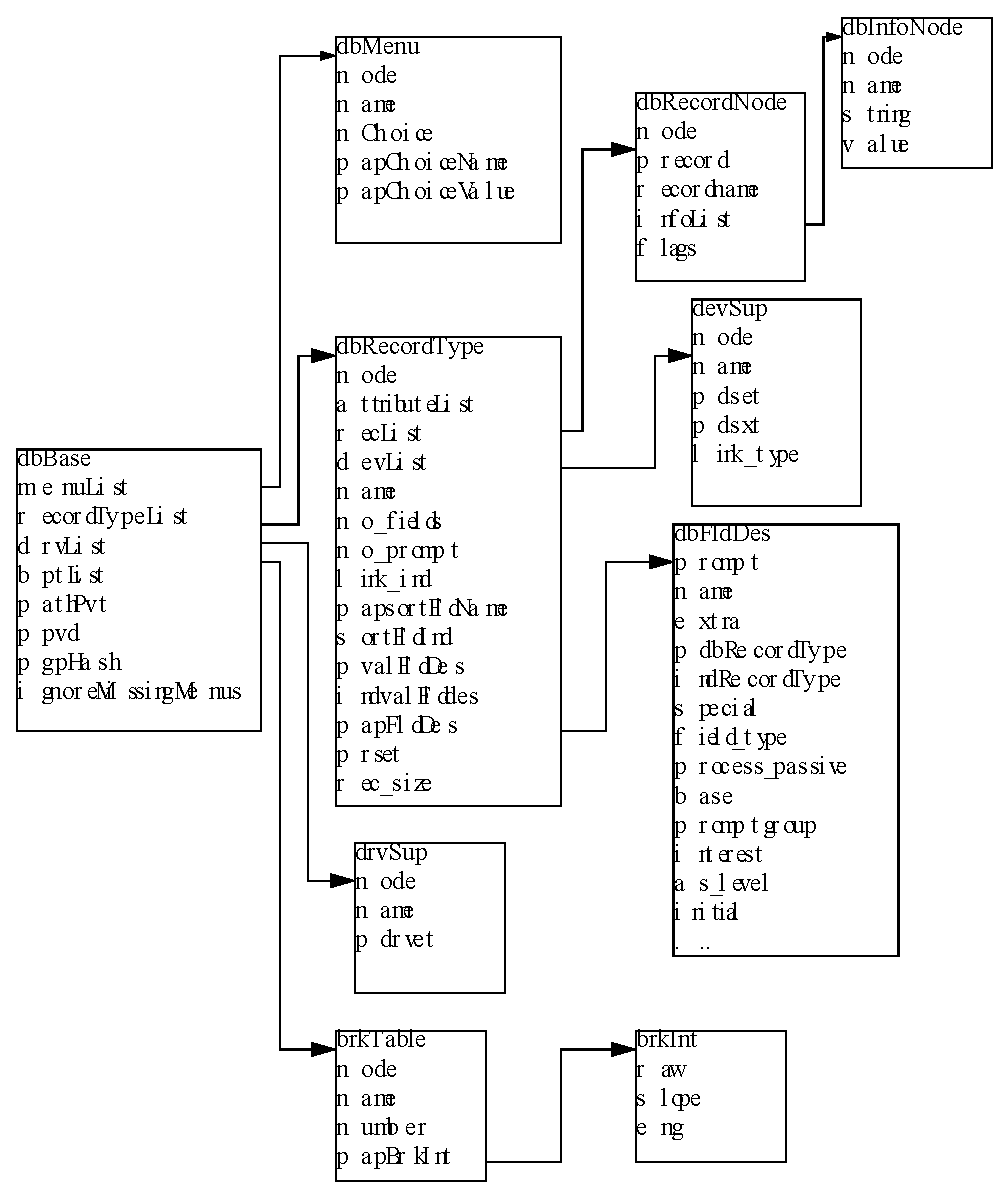
\includegraphics{databaseStructures_1}








